%==============================================================================
% Sjabloon onderzoeksvoorstel bachproef
%==============================================================================
% Gebaseerd op document class `hogent-article'
% zie <https://github.com/HoGentTIN/latex-hogent-article>

% Voor een voorstel in het Engels: voeg de documentclass-optie [english] toe.
% Let op: kan enkel na toestemming van de bachelorproefcoördinator!
\documentclass{hogent-article}

% Invoegen bibliografiebestand
\addbibresource{voorstel.bib}

% Pakketten voor figuren en flowchart
\usepackage{graphicx}
\usepackage{tikz}
\usetikzlibrary{shapes.geometric, arrows, positioning}

% Informatie over de opleiding, het vak en soort opdracht
\studyprogramme{Professionele bachelor toegepaste informatica}
\course{Bachelorproef}
\assignmenttype{Onderzoeksvoorstel}
% Voor een voorstel in het Engels, haal de volgende 3 regels uit commentaar
% \studyprogramme{Bachelor of applied information technology}
% \course{Bachelor thesis}
% \assignmenttype{Research proposal}

\academicyear{2025-2026}

% TODO: Werktitel
\title{Beveiliging van AI‑agents in Fintech: automatische detectie van beveiligingslekken in integraties op basis van het Model Context Protocol (MCP)}

\author{Arthur Van Oudenhove}
\email{arthur.vanoudenhove@student.hogent.be}
\projectrepo{https://github.com/Arthur-VO/bachelorproef} 

% TODO: Geef de co-promotor op
\supervisor[Co-promotor]{/}

% Binnen welke specialisatierichting uit 3TI situeert dit onderzoek zich?
% Kies uit deze lijst:
%
% - Mobile \& Enterprise development
% - AI \& Data Engineering
% - Functional \& Business Analysis
% - System \& Network Administrator
% - Mainframe Expert
% - Als het onderzoek niet past binnen een van deze domeinen specifieer je deze
%   zelf
%
\specialisation{AI \& Data Engineering}
\keywords{MCP, AI, Security, Fintech}

\begin{document}

\begin{abstract}
%  Hier schrijf je de samenvatting van je voorstel, als een doorlopende tekst van één paragraaf. Let op: dit is geen inleiding, maar een samenvattende tekst van heel je voorstel met inleiding (voorstelling, kaderen thema), probleemstelling en centrale onderzoeksvraag, onderzoeksdoelstelling (wat zie je als het concrete resultaat van je bachelorproef?), voorgestelde methodologie, verwachte resultaten en meerwaarde van dit onderzoek (wat heeft de doelgroep aan het resultaat?).
    Binnen de Fintech-sector neemt de integratie van AI-agents in de bedrijfsvoering structureel toe. Deze agents worden ingezet voor bedrijfskritische processen, waarbij een 'proces' gedefinieerd wordt als een reeks handelingen die een specifiek zakelijk doel dienen. Een proces is 'kritiek' wanneer een beveiligingsincident direct leidt tot aanzienlijke financiële schade, reputatieverlies of het stopzetten van de dienstverlening.

    Het Model Context Protocol (MCP) vormt hierbij de technische interface die AI-modellen verbindt met databronnen. Hoewel MCP operationele voordelen biedt, is er momenteel een kennistekort over de effectiviteit van bestaande beveiligingsmethoden voor dit specifieke protocol. Dit onderzoek richt zich op de vraag in welke mate een geautomatiseerd framework de detectiegraad van protocol-specifieke kwetsbaarheden — zoals prompt injection, tool poisoning en privilege escalation — kan verbeteren ten opzichte van de huidige handmatige controleprocessen.

    Om dit te onderzoeken, wordt een geautomatiseerd security assessment framework ontworpen en geïmplementeerd als onderzoeksinstrument. Dit framework dient als testomgeving om de betrouwbaarheid en schaalbaarheid van geautomatiseerde inspectieprotocollen te toetsen. Door middel van een Proof of Concept (PoC) worden kwantitatieve data verzameld over de detectie-efficiëntie en de reductie in doorlooptijd van beveiligingsbeoordelingen (security reviews).

    De resultaten van dit onderzoek bieden niet alleen een werkende oplossing, maar genereren fundamentele inzichten in de beperkingen van handmatige audits en de randvoorwaarden voor veilige MCP-integraties. Hiermee levert de studie onderbouwde conclusies op over de haalbaarheid van een systematische beveiligingsaanpak binnen Fintech-organisaties, die verder gaan dan de loutere technische implementatie.
\end{abstract}

\tableofcontents

% De hoofdtekst van het voorstel zit in een apart bestand, zodat het makkelijk
% kan opgenomen worden in de bijlagen van de bachelorproef zelf.
song2025protocolunveilingattackvectors%---------- Inleiding ---------------------------------------------------------

% TODO: Is dit voorstel gebaseerd op een paper van Research Methods die je
% vorig jaar hebt ingediend? Heb je daarbij eventueel samengewerkt met een
% andere student?
% Zo ja, haal dan de tekst hieronder uit commentaar en pas aan.

%\paragraph{Opmerking}

% Dit voorstel is gebaseerd op het onderzoeksvoorstel dat werd geschreven in het
% kader van het vak Research Methods dat ik (vorig/dit) academiejaar heb
% uitgewerkt (met medesturent VOORNAAM NAAM als mede-auteur).
% 

\section{Inleiding}%
\label{sec:inleiding}

De sector van financiële technologie, of Fintech, ontwikkelt zich razendsnel. Dat komt door de adoptie van autonome AI-agents. Deze slimme systemen doen niet alleen simpele klussen. Ze nemen complexere processen over. Van het afhandelen van klantvragen tot het verwerken van terugbetalingen en transacties. Voor effectieve communicatie met interne databases en API's is het Model Context Protocol essentieel. MCP zorgt voor interoperabiliteit als standaard.

Deze vooruitgang in technologie heeft een nadeel. Het verhoogt de veiligheidsrisico's aanzienlijk en die worden groter. Neem een Fintech-startup die een AI-agent via MCP toegang geeft tot betaalsystemen. Dat opent nieuwe wegen voor aanvallen. Kwaadwillenden kunnen prompt injection gebruiken om instructies van de agent te veranderen. Of tool poisoning om slechte commando's in data te verbergen. Gevolgen variëren van datalekken tot privilege escalation. Daarmee krijgt een agent bijvoorbeeld per ongeluk admin-rechten.\autocite{song2025protocolunveilingattackvectors}

Security-teams hebben vaak niet genoeg middelen om MCP-implementaties goed te beschermen. De praktijk hangt af van handmatige code-reviews en tijdelijke tools. Die tools passen niet bij de details van MCP. Dit maakt een knelpunt. Innovatie vertraagt door lange checks. Of servers gaan online zonder echte controle, wat vaker gebeurt. Onderzoek toont de urgentie. Zesenvijftig procent van de bedrijven met AI-agents meldt lekken in MCP-omgevingen, \autocite{guo2025systematicanalysismcpsecurity}. Dit voorstel pakt die kloof aan met automatisering en standaardisatie.




%\begin{itemize}
%  \item kaderen thema
%  \item de doelgroep
%  \item de probleemstelling en (centrale) onderzoeksvraag
%  \item de onderzoeksdoelstelling
%\end{itemize}
%
%Denk er aan: een typische bachelorproef is \textit{toegepast onderzoek}, wat betekent dat je start vanuit een concrete probleemsituatie in bedrijfscontext, een \textbf{casus}. Het is belangrijk om je onderwerp goed af te bakenen: je gaat voor die \textit{ene specifieke probleemsituatie} op zoek naar een goede oplossing, op basis van de huidige kennis in het vakgebied.
%
%De doelgroep moet ook concreet en duidelijk zijn, dus geen algemene of vaag gedefinieerde groepen zoals \emph{bedrijven}, \emph{developers}, \emph{Vlamingen}, enz. Je richt je in elk geval op it-professionals, een bachelorproef is geen populariserende tekst. Eén specifiek bedrijf (die te maken hebben met een concrete probleemsituatie) is dus beter dan \emph{bedrijven} in het algemeen.
%
%Formuleer duidelijk de onderzoeksvraag! De begeleiders lezen nog steeds te veel voorstellen waarin we geen onderzoeksvraag terugvinden.
%
%Schrijf ook iets over de doelstelling. Wat zie je als het concrete eindresultaat van je onderzoek, naast de uitgeschreven scriptie? Is het een proof-of-concept, een rapport met aanbevelingen, \ldots Met welk eindresultaat kan je je bachelorproef als een succes beschouwen?
%


\section{Probleemstelling}
\label{sec:probleemstelling}

Het kernprobleem is dat Fintech-bedrijven momenteel geen gestructureerde en geautomatiseerde manier hebben om MCP-servers op kritieke veiligheidskwetsbaarheden te controleren vóór live-gang.

\begin{itemize}
    \item \textbf{Huidige situatie (Status Quo):} Security teams vertrouwen op handmatige code reviews, wat een bottleneck vormt en vaak onvolledig is. Er wordt gebruikgemaakt van ad-hoc tools zoals Burp Suite of Semgrep, maar deze missen specifieke context voor MCP-gerelateerde aanvallen.
    \item \textbf{Specifieke risico's:} Zonder degelijke screening zijn servers kwetsbaar voor:
    \begin{itemize}
        \item \emph{Prompt injection attacks} via manipulatie van tool-beschrijvingen.
        \item \emph{Token theft \& privilege escalation}, waarbij agents te brede rechten krijgen.
        \item \emph{Tool poisoning}, waarbij kwaadaardige instructies in data worden verstopt.
        \item \emph{Confused deputy attacks}, omdat servers vaak geen onderscheid maken tussen gebruikers.
        \item Gebrek aan \emph{audit logging}, waardoor acties niet traceerbaar zijn.
    \end{itemize}
    \item \textbf{Doelgroep:} Het onderzoek richt zich op security teams, DevSecOps-engineers en enterprise architects binnen Fintech, e-commerce en andere gereguleerde industrieën.
\end{itemize}

\section{Doelstelling}
\label{sec:doelstelling}

Deze bachelorproef wil een geautomatiseerd security assessment framework ontwerpen, ontwikkelen en valideren. Het richt zich op MCP-servers. De resultaten zijn concreet voor MCP-servers.
\begin{enumerate}
    \item Een werkend prototype (Proof-of-Concept) van de security scanner.
    \item Een validatie van de effectiviteit van dit framework ten opzichte van handmatige reviews (detectiegraad en tijdsbesparing).
    \item Een set aanbevelingen voor de veilige implementatie van MCP in bedrijfsomgevingen.
\end{enumerate}

\section{Onderzoeksvragen}
\label{sec:onderzoeksvragen}

\paragraph{Hoofdvraag}
Hoe kan een geautomatiseerd security assessment framework ontworpen en geïmplementeerd worden om MCP-server implementaties in bedrijfsomgevingen systematischer en efficiënter te screenen op kritieke kwetsbaarheden dan de huidige handmatige processen?

\paragraph{Deelvragen Probleemdomein}
\begin{enumerate}
    \item Hoeveel van de top 10 MCP-kwetsbaarheden worden momenteel gedetecteerd door handmatige security reviews binnen fintech-bedrijven?
    \item Wat is het percentage MCP-implementaties in enterprises die kwetsbaar zijn voor prompt injection attacks, zoals vastgesteld door recent gepubliceerde onderzoeken?
    \item Hoe vaak leiden MCP-gerelateerde kwetsbaarheden in de praktijk tot datalekken of frauduleuze transacties (incidentratio in de laatste 24 maanden)?
    \item Hoeveel tijd besteden security teams gemiddeld aan het handmatig screenen van MCP-server code?
    \item Wat is het percentage false negatives bij bestaande handmatige controles?
\end{enumerate}

\paragraph{Deelvragen Oplossingsdomein}
\begin{enumerate}
    \item Hoeveel procent van de MCP-kwetsbaarheden kan een geautomatiseerde tool detecteren in vergelijking met handmatige reviews?
    \item Wat is de gemiddelde tijdsbesparing bij het scannen van MCP-servers door een geautomatiseerde pipeline?
    \item Wat is het percentage false positives/negatives bij gebruik van SAST, DAST en fuzzing op MCP-implementaties?
    \item Hoeveel MCP-servers kunnen effectief per dag worden gescand met het voorgestelde framework?
    \item Hoe verbeteren geprioriteerde rapporten de reactietijd van security teams?
\end{enumerate}


%---------- Stand van zaken ---------------------------------------------------

\section{Literatuurstudie}%
\label{sec:literatuurstudie}

\subsection{Opkomst en risico's van MCP in Fintech}

De integratie van AI-agents in de financiële sector, voor toepassingen variërend van klantenservice tot transactieverwerking, steunt in toenemende mate op gestandaardiseerde protocollen. Het Model Context Protocol (MCP) fungeert hierbij als een kritieke brug tussen AI-modellen en bedrijfsapplicaties met toebehorende data. Hoewel deze standaardisatie integratie vergemakkelijkt, hebben \textcite{song2025protocolunveilingattackvectors} aangetoond dat het ecosysteem hierdoor nieuwe aanvalsvectoren introduceert die verder reiken dan het protocol zelf.

De complexiteit van deze implementaties brengt specifieke beveiligingsrisico's met zich mee. Uit een systematische analyse door \textcite{guo2025systematicanalysismcpsecurity} blijkt dat MCP-implementaties vatbaar zijn voor diverse fundamentele kwetsbaarheden, waaronder \emph{prompt injection} via tool-beschrijvingen en \emph{privilege escalation}. In de praktijk kunnen kwaadwillenden deze zwakheden exploiteren. Zo beschrijven \textcite{Cato2025} in hun onderzoek naar "Living off AI"-aanvallen hoe MCP-servers gemanipuleerd kunnen worden omdat ze onvoldoende onderscheid maken tussen legitieme gebruikers en externe actoren, ook wel bekend als de \emph{confused deputy} aanval.

\subsection{Classificatie van kwetsbaarheden}

Om de grote hoeveelheid aan risico's te categoriseren, zijn er initiatieven gestart om de meest kritieke lekken in kaart te brengen. \textcite{OWASP2025} hebben een lijst van de "Top 10 MCP vulnerabilities" opgesteld, waarin onder andere \emph{tool poisoning} en het gebrek aan degelijke audit logging als prominente risico's worden bestempeld. Voor fintech-bedrijven, die met gevoelige persoons- en transactiegegevens werken, vormen deze specifieke kwetsbaarheden een direct risico op datalekken en compliance-schendingen.

\subsection{Status Quo: Beperkingen van handmatige validatie}

Ondanks de ernst van de dreigingen, ontbreken er momenteel gestandaardiseerde methodologieën voor validatie. De huidige praktijk in het bedrijfsleven leunt sterk op handmatige en herhaalde code reviews en het gebruik van ad-hoc tools. \textcite{Uproot2025} bieden weliswaar handleidingen voor het uitvoeren van MCP-pentests, maar deze processen blijven arbeidsintensief en foutgevoelig, wat het tijdsaspect dus niet positief beïnvloedt.

Bestaande tools bieden slechts gedeeltelijke oplossingen. Hoewel er open-source initiatieven zijn, zoals de scanning tool van \textcite{Invariant2025}, ontbreekt vaak een integratie in een breder security framework dat geschikt is voor enterprise-omgevingen. Bedrijven vallen hierdoor vaak terug op algemene tools zoals Burp Suite of Semgrep die de context-specifieke logica van MCP niet volledig begrijpen. Dit leidt tot een situatie waarin, volgens marktobservaties, een aanzienlijk deel van de deployments live gaat met niet-gedetecteerde veiligheidslekken.

Het ontbreken van een geautomatiseerd, gestructureerd framework dat specifiek is ontworpen voor de nuances van MCP-servers, vormt het centrale onderwerp in de huidige literatuur en praktijk. Dit onderzoek beoogt dit gat te dichten door een dergelijk framework te ontwerpen en de effectiviteit hiervan te evalueren.


%Hier beschrijf je de \emph{state-of-the-art} rondom je gekozen onderzoeksdomein, d.w.z.\ een inleidende, doorlopende tekst over het onderzoeksdomein van je bachelorproef. Je steunt daarbij heel sterk op de professionele \emph{vakliteratuur}, en niet zozeer op populariserende teksten voor een breed publiek. Wat is de huidige stand van zaken in dit domein, en wat zijn nog eventuele open vragen (die misschien de aanleiding waren tot je onderzoeksvraag!)?
%
%Je mag de titel van deze sectie ook aanpassen (literatuurstudie, stand van zaken, enz.). Zijn er al gelijkaardige onderzoeken gevoerd? Wat concluderen ze? Wat is het verschil met jouw onderzoek?
%
%Verwijs bij elke introductie van een term of bewering over het domein naar de vakliteratuur, bijvoorbeeld~\autocite{Hykes2013}! Denk zeker goed na welke werken je refereert en waarom.
%
%Draag zorg voor correcte literatuurverwijzingen! Een bronvermelding hoort thuis \emph{binnen} de zin waar je je op die bron baseert, dus niet er buiten! Maak meteen een verwijzing als je gebruik maakt van een bron. Doe dit dus \emph{niet} aan het einde van een lange paragraaf. Baseer nooit teveel aansluitende tekst op eenzelfde bron.
%
%Als je informatie over bronnen verzamelt in JabRef, zorg er dan voor dat alle nodige info aanwezig is om de bron terug te vinden (zoals uitvoerig besproken in de lessen Research Methods).
%
% Voor literatuurverwijzingen zijn er twee belangrijke commando's:
% \autocite{KEY} => (Auteur, jaartal) Gebruik dit als de naam van de auteur
%   geen onderdeel is van de zin.
% \textcite{KEY} => Auteur (jaartal)  Gebruik dit als de auteursnaam wel een
%   functie heeft in de zin (bv. ``Uit onderzoek door Doll & Hill (1954) bleek
%   ...'')

Je mag deze sectie nog verder onderverdelen in subsecties als dit de structuur van de tekst kan verduidelijken.

%---------- Methodologie ------------------------------------------------------
\section{Methodologie}%
\label{sec:methodologie}

Om objectieve en meetbare resultaten te garanderen, worden subjectieve methoden zoals enquêtes vermeden. In plaats daarvan wordt gekozen voor experimentele validatie aan de hand van kwantitatieve metrieken. Figuur~\ref{fig:methodologie_flow} geeft een schematisch overzicht van de doorlopen fasen.

% --- TIKZ FLOWCHART ---
\begin{figure*}[htbp]
\centering
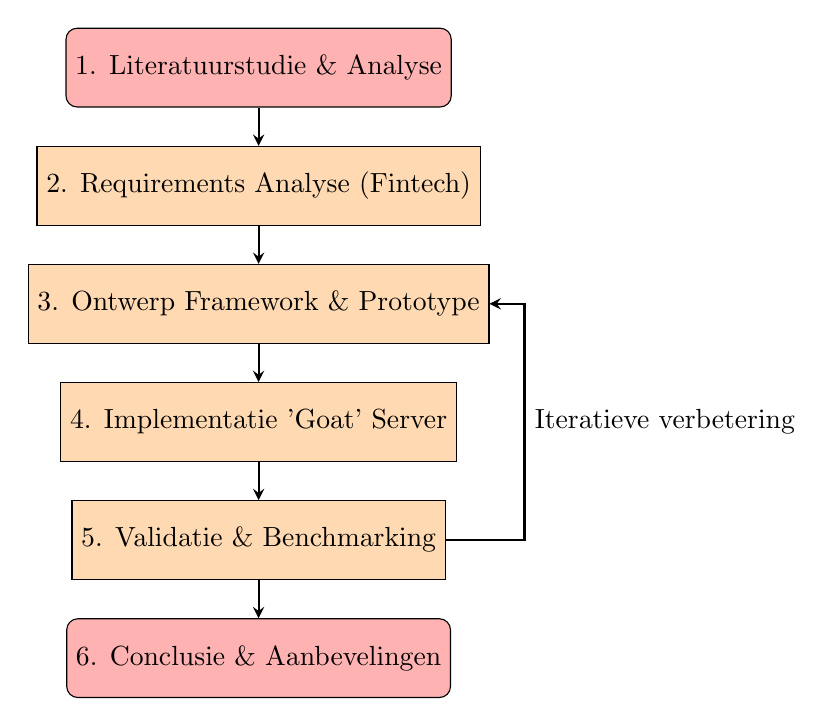
\begin{tikzpicture}[node distance=1.5cm]
    % Stijlen definiëren
    \tikzstyle{startstop} = [rectangle, rounded corners, minimum width=3cm, minimum height=1cm, text centered, draw=black, fill=red!30]
    \tikzstyle{process} = [rectangle, minimum width=3cm, minimum height=1cm, text centered, draw=black, fill=orange!30]
    \tikzstyle{io} = [trapezium, trapezium left angle=70, trapezium right angle=110, minimum width=3cm, minimum height=1cm, text centered, draw=black, fill=blue!30]
    \tikzstyle{arrow} = [thick,->,>=stealth]

    % Knopen plaatsen
    \node (lit) [startstop] {1. Literatuurstudie \& Analyse};
    \node (req) [process, below of=lit] {2. Requirements Analyse (Fintech)};
    \node (design) [process, below of=req] {3. Ontwerp Framework \& Prototype};
    \node (poc) [process, below of=design] {4. Implementatie 'Goat' Server};
    \node (test) [process, below of=poc] {5. Validatie \& Benchmarking};
    \node (concl) [startstop, below of=test] {6. Conclusie \& Aanbevelingen};

    % Pijlen trekken
    \draw [arrow] (lit) -- (req);
    \draw [arrow] (req) -- (design);
    \draw [arrow] (design) -- (poc);
    \draw [arrow] (poc) -- (test);
    \draw [arrow] (test) -- (concl);
    
    % Feedback loop
    \draw [arrow] (test.east) -- ++(1,0) |- (design.east) node[pos=0.25, right] {Iteratieve verbetering};

\end{tikzpicture}
\caption{Schematische weergave van de onderzoeksstappen.}
\label{fig:methodologie_flow}
\end{figure*}

\subsection{Fase 1: Literatuurstudie en classificatie van dreigingen}

\textbf{Onderzoekstechniek:} Literatuurstudie. \\
Het onderzoek start met een diepgaande analyse van de technische specificaties van het Model Context Protocol (MCP). Er wordt gebruikgemaakt van academische databanken (zoals Google Scholar, IEEE Xplore en arXiv) en officiële technische documentatie om de architectuur en datastromen te doorgronden. Specifiek wordt gezocht naar bestaande taxonomieën van AI-kwetsbaarheden (zoals de OWASP Top 10 voor LLM's) en hoe deze zich vertalen naar de MCP-context.

\textbf{Doel:} Het opstellen van een specifieke taxonomie van kwetsbaarheden (zoals prompt injection, tool poisoning en privilege escalation) die relevant zijn voor de financiële sector. 

\textbf{Tools:} BiBTex voor referentiebeheer, LaTeX voor documentatie. \\
\textbf{Tijdschatting:} 4 weken. \\
\textbf{Deliverable:} Hoofdstuk 'Literatuurstudie' met een gedefinieerd dreigingsmodel.

\subsection{Fase 2: Requirementsanalyse voor Fintech-toepassingen}

\textbf{Onderzoekstechniek:} Documentanalyse en functionele analyse. \\
In plaats van interviews of enquêtes, die subjectieve meningen opleveren, wordt er gekeken naar harde compliance-eisen uit de financiële sector (zoals PCI-DSS en GDPR) en best practices voor API-security. Op basis hiervan worden de functionele en niet-functionele vereisten (zoals logging, auditability en toegangscontrole) voor de scanner vastgelegd volgens de MoSCoW-methode.

\textbf{Doel:} Een objectieve lijst van criteria opstellen waaraan het te ontwikkelen framework moet voldoen om inzetbaar te zijn in een enterprise-omgeving.

\textbf{Tools:} Requirements management templates. \\
\textbf{Tijdschatting:} 2 weken. \\
\textbf{Deliverable:} Een geprioriteerde lijst van requirements.

\subsection{Fase 3: Ontwerp en implementatie van het assessment framework}

\textbf{Onderzoekstechniek:} Prototyping en iteratieve softwareontwikkeling (PoC). \\
Dit is de technisch meest complexe fase waarin het artefact daadwerkelijk wordt gebouwd. De scanner wordt modulair opgezet om flexibiliteit te garanderen. De technische realisatie gebeurt in Python vanwege de uitgebreide ondersteuning voor JSON-RPC en asynchrone communicatie, essentieel voor MCP.

Het framework bestaat uit drie kerncomponenten:
\begin{enumerate}
    \item \textbf{Discovery Module:} Analyseert de \texttt{list\_tools} en \texttt{list\_prompts} endpoints.
    \item \textbf{Static Analysis Engine:} Scant tool-beschrijvingen op onveilige patronen.
    \item \textbf{Dynamic Probing Engine:} Voert actieve fuzzing uit met gemanipuleerde payloads.
\end{enumerate}

\textbf{Tools:} Python 3.12+, Docker (voor containerisatie), Git (versiebeheer), Pydantic (data validatie), `mcp`-library. \\
\textbf{Tijdschatting:} 6 weken. \\
\textbf{Deliverable:} Een werkende Proof of Concept (PoC) van de scanner, gepubliceerd als open-source code op GitHub.

\subsection{Fase 4: Validatie via een 'Vulnerable MCP Server'}

\textbf{Onderzoekstechniek:} Experimentele validatie en vergelijkende studie. \\
Omdat er weinig publieke testdata is, wordt een eigen testomgeving ontwikkeld: de 'Fintech MCP Goat'. Dit is een opzettelijk onveilige MCP-server die financiële use-cases nabootst (bv. saldo opvragen, overschrijving starten). 

Deze omgeving dient als 'ground truth'. De effectiviteit van de scanner wordt gemeten door deze los te laten op de 'Goat' server en de resultaten te vergelijken met de bekende kwetsbaarheden. De validatie is puur kwantitatief:
\begin{itemize}
    \item \textbf{Detectieratio (Recall):} $\frac{\text{Aantal gevonden kwetsbaarheden}}{\text{Totaal aantal aanwezige kwetsbaarheden}}$
    \item \textbf{False Positive Rate:} Aantal onterechte alarmen.
    \item \textbf{Performance:} Scan-tijd in milliseconden.
\end{itemize}

\textbf{Tools:} Docker Compose (voor het opzetten van de testlab), Pytest (voor geautomatiseerde testsuites), Burp Suite (voor manuele verificatie van bevindingen). \\
\textbf{Tijdschatting:} 3 weken. \\
\textbf{Deliverable:} Validatierapport met meetresultaten en een analyse van de nauwkeurigheid.

\subsection{Overzichtstabel Planning}

Tabel~\ref{tab:planning} geeft een samenvattend overzicht van de fasering en deliverables.

\begin{table*}[htbp]
\centering
\caption{Planning en deliverables per onderzoeksfase.}
\label{tab:planning}
\begin{tabular}{@{}llp{6cm}@{}}
\toprule
\textbf{Fase} & \textbf{Duur} & \textbf{Deliverable} \\ \midrule
1. Literatuurstudie & 4 weken & Dreigingsmodel \& State-of-the-art \\
2. Requirements & 2 weken & Requirementslijst (MoSCoW) \\
3. Implementatie & 6 weken & Python Framework (GitHub repo) \\
4. Validatie & 3 weken & Validatierapport \& Testresultaten \\
5. Conclusie & 2 weken & Finaliseren Bachelorproef tekst \\ \bottomrule
\end{tabular}
\end{table*}

%Hier beschrijf je hoe je van plan bent het onderzoek te voeren. Welke onderzoekstechniek ga je toepassen om elk van je onderzoeksvragen te beantwoorden? Gebruik je hiervoor literatuurstudie, interviews met belanghebbenden (bv.~voor requirements-analyse), experimenten, simulaties, vergelijkende studie, risico-analyse, PoC, \ldots?
%
%Valt je onderwerp onder één van de typische soorten bachelorproeven die besproken zijn in de lessen Research Methods (bv.\ vergelijkende studie of risico-analyse)? Zorg er dan ook voor dat we duidelijk de verschillende stappen terug vinden die we verwachten in dit soort onderzoek!
%
%Vermijd onderzoekstechnieken die geen objectieve, meetbare resultaten kunnen opleveren. Enquêtes, bijvoorbeeld, zijn voor een bachelorproef informatica meestal \textbf{niet geschikt}. De antwoorden zijn eerder meningen dan feiten en in de praktijk blijkt het ook bijzonder moeilijk om voldoende respondenten te vinden. Studenten die een enquête willen voeren, hebben meestal ook geen goede definitie van de populatie, waardoor ook niet kan aangetoond worden dat eventuele resultaten representatief zijn.
%
%Uit dit onderdeel moet duidelijk naar voor komen dat je bachelorproef ook technisch voldoen\-de diepgang zal bevatten. Het zou niet kloppen als een bachelorproef informatica ook door bv.\ een student marketing zou kunnen uitgevoerd worden.
%
%Je beschrijft ook al welke tools (hardware, software, diensten, \ldots) je denkt hiervoor te gebruiken of te ontwikkelen.
%
%Probeer ook een tijdschatting te maken. Hoe lang zal je met elke fase van je onderzoek bezig zijn en wat zijn de concrete \emph{deliverables} in elke fase?
%


%---------- Verwachte resultaten ----------------------------------------------
\section{Verwacht resultaat, conclusie}%
\label{sec:verwachte_resultaten}

\subsection{Verwachte prestaties van het framework}

Het belanrijkste verwachte resultaat is een functionerend prototype (de scanner) dat in staat is om de in de literatuurstudie geïdentificeerde top-kwetsbaarheden autonoom te detecteren. Er worden twee specifieke meetbare uitkomsten verwacht: een verhoogde detectieconsistentie en een significante tijdsbesparing.

\subsubsection{Hypothese 1: Detectieratio en Dekking}
De verwachting is dat het geautomatiseerde framework een hogere en consistentere detectieratio (Recall) behaalt voor technische kwetsbaarheden (zoals \emph{Prompt Injection} en onveilige \emph{Tool Definitions}) dan een gemiddelde handmatige review.

Figuur~\ref{fig:mockup_detectie} toont de verwachte verdeling van de detectieresultaten. Op de Y-as staat het percentage gedetecteerde kwetsbaarheden (Detectieratio), en op de X-as de verschillende categorieën van MCP-risico's.

\begin{figure*}[htbp]
    \centering
    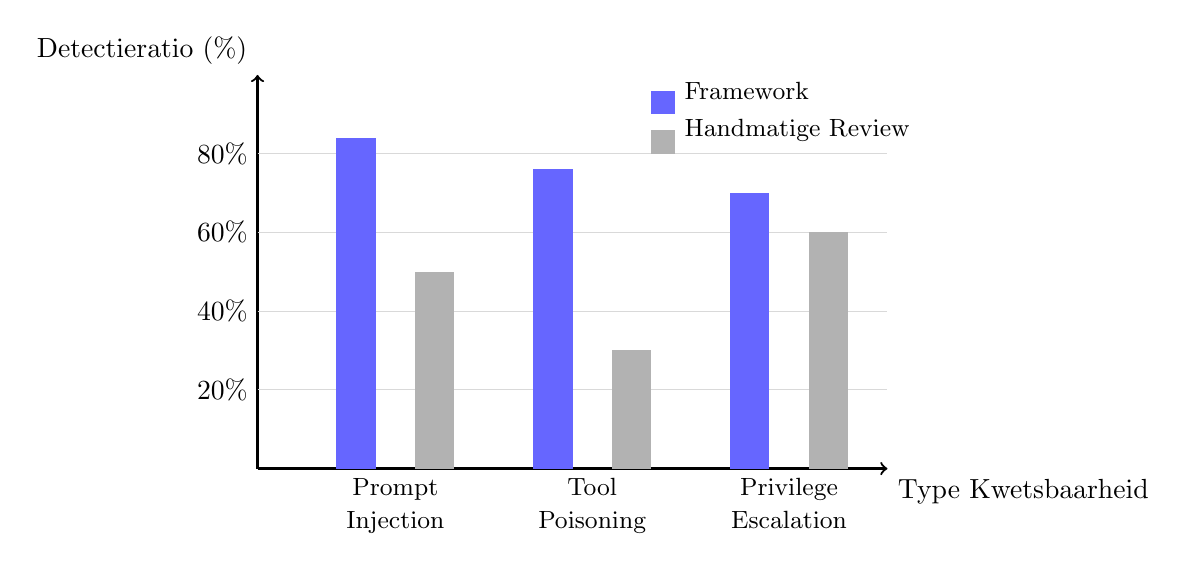
\begin{tikzpicture}
        % Assen
        \draw[thick,->] (0,0) -- (8,0) node[anchor=north west] {Type Kwetsbaarheid};
        \draw[thick,->] (0,0) -- (0,5) node[anchor=south east] {Detectieratio (\%)};
        
        % Grid en labels Y-as
        \foreach \y/\label in {1/20, 2/40, 3/60, 4/80} {
            \draw[gray!30] (0,\y) -- (8,\y);
            \node[left] at (0,\y) {\label\%};
        }
        
        % Labels X-as
        \node[below, align=center] at (1.75,0) {\small Prompt\\ \small Injection};
        \node[below, align=center] at (4.25,0) {\small Tool\\ \small Poisoning};
        \node[below, align=center] at (6.75,0) {\small Privilege\\ \small Escalation};

        % Data (Mock-up) - Blauw = Framework, Grijs = Handmatig
        % Prompt Injection
        \fill[blue!60] (1.0,0) rectangle (1.5, 4.2); % Framework (hoog)
        \fill[gray!60] (2.0,0) rectangle (2.5, 2.5); % Handmatig (lager/wisselend)
        
        % Tool Poisoning
        \fill[blue!60] (3.5,0) rectangle (4.0, 3.8); 
        \fill[gray!60] (4.5,0) rectangle (5.0, 1.5); % Handmatig mist dit vaak
        
        % Priv Escalation
        \fill[blue!60] (6.0,0) rectangle (6.5, 3.5); 
        \fill[gray!60] (7.0,0) rectangle (7.5, 3.0); 

        % Legenda
        \fill[blue!60] (5,4.5) rectangle (5.3,4.8) node[right, black] {\small Framework};
        \fill[gray!60] (5,4.0) rectangle (5.3,4.3) node[right, black] {\small Handmatige Review};
    \end{tikzpicture}
    \caption{Mock-up: Verwachte detectieratio van het framework t.o.v. handmatige review. We verwachten dat het framework vooral beter scoort op complexe, technische patronen zoals Tool Poisoning.}
    \label{fig:mockup_detectie}
\end{figure*}

De motivatie achter deze verwachting is dat statische analyse-engines (SAST) in staat zijn om duizenden regels code en configuratiebestanden te scannen op patronen die voor het menselijk oog moeilijk te vinden zijn, zeker wanneer deze verspreid zijn over meerdere bestanden. Wel wordt verwacht dat het aantal \emph{False Positives} (onterechte alarmen) bij het framework initieel hoger zal liggen dan bij een menselijke expert, wat in de discussie genuanceerd zal moeten worden.

\subsubsection{Hypothese 2: Tijdsbesparing en Schaalbaarheid}
Een tweede belangrijke verwachting is de schaalbaarheid. Figuur~\ref{fig:mockup_tijd} visualiseert de verwachte tijdsbesteding. Op de X-as staat de complexiteit van de MCP-server (aantal tools/endpoints), en op de Y-as de benodigde tijd voor een security assessment.

\begin{figure*}[htbp]
    \centering
    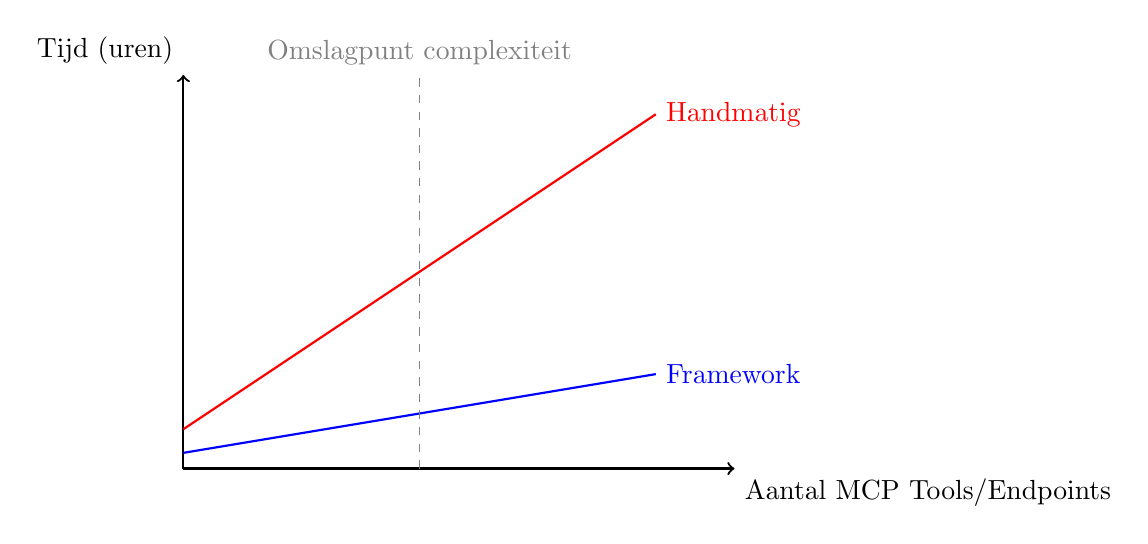
\begin{tikzpicture}
        % Assen
        \draw[thick,->] (0,0) -- (7,0) node[anchor=north west] {Aantal MCP Tools/Endpoints};
        \draw[thick,->] (0,0) -- (0,5) node[anchor=south east] {Tijd (uren)};
        
        % Lijnen tekenen
        % Handmatig (Lineair steil)
        \draw[red, thick] (0,0.5) -- (6,4.5) node[right] {Handmatig};
        % Framework (Vlakker)
        \draw[blue, thick] (0,0.2) -- (6,1.2) node[right] {Framework};
        
        % Stippellijnen voor threshold
        \draw[dashed, gray] (3,0) -- (3,5);
        \node[above, gray] at (3,5) {Omslagpunt complexiteit};

    \end{tikzpicture}
    \caption{Mock-up: Verwachte tijdsbesteding. Naarmate de complexiteit van de MCP-server toeneemt, blijft de scantijd van het framework nagenoeg constant, terwijl handmatige review lineair toeneemt.}
    \label{fig:mockup_tijd}
\end{figure*}

De verwachting is dat het framework een volledige scan kan uitvoeren in enkele minuten, ongeacht of de server 5 of 50 tools definieert. Dit staat in contrast met handmatige penetratietesten, die dagen in beslag kunnen nemen.

\subsection{Meerwaarde voor de doelgroep}

Voor Fintech-bedrijven, de primaire doelgroep, biedt dit resultaat drie concrete voordelen:
\begin{enumerate}
    \item \textbf{Continuous Compliance:} Door de scanner te integreren in de CI/CD-pijplijn, kunnen bedrijven bij elke code-wijziging aantonen dat de AI-agents nog steeds voldoen aan veiligheidseisen. Dit is cruciaal voor audits (bv. SOC2 of DORA).
    \item \textbf{Time-to-Market:} Security wordt geen bottleneck meer. Ontwikkelaars krijgen directe feedback over onveilige tool-definities zonder te moeten wachten op een beschikbaar security-team.
    \item \textbf{Risicoreductie:} Door veelvoorkomende kwetsbaarheden zoals \emph{Confused Deputy} aanvallen automatisch af te vangen, verkleint de kans op fraude en datalekken via AI-interfaces aanzienlijk.
\end{enumerate}

\subsection{Conclusie}
Dit onderzoek toont aan dat een gespecialiseerd security framework voor MCP haalbaar en nodig is. Voor veilige AI-agents in financiën.

Als resultaten afwijken, zoals te weinig context voor complexe fouten, is dat ook waardevol. Het wijst op afhankelijkheid van menselijke expertise. En noodzaak voor hybrid approach in de nabije toekomst.



%Hier beschrijf je welke resultaten je verwacht. Als je metingen en simulaties uitvoert, kan je hier al mock-ups maken van de grafieken samen met de verwachte conclusies. Benoem zeker al je assen en de onderdelen van de grafiek die je gaat gebruiken. Dit zorgt ervoor dat je concreet weet welk soort data je moet verzamelen en hoe je die moet meten.
%
%Wat heeft de doelgroep van je onderzoek aan het resultaat? Op welke manier zorgt jouw bachelorproef voor een meerwaarde?
%
%Hier beschrijf je wat je verwacht uit je onderzoek, met de motivatie waarom. Het is \textbf{niet} erg indien uit je onderzoek andere resultaten en conclusies vloeien dan dat je hier beschrijft: het is dan juist interessant om te onderzoeken waarom jouw hypothesen niet overeenkomen met de resultaten.
%


\printbibliography[heading=bibintoc]

\end{document}